\providecommand{\main}{../../../..}
\documentclass[\main/dresen_thesis.tex]{subfiles}
\renewcommand{\thisPath}{\main/chapters/theoreticalBackground/ferrites/cobaltferrite}
\begin{document}

\subsection{Cobalt Ferrite}\label{ch:theoreticalBackground:cobaltferrite}
  Bulk cobalt ferrite (\ch{CoFe2O4}) is a ferrimagnetic material with a high cubic magnetocrystalline anisotropy and moderate saturation magnetization.
  Due to its high thermal/chemical stability, magnetic properties and cheap production costs, it is of interest for practical use \textit{i.e.} in high-density magnetic recording \cite{Wu_2014_Monol}, magneto-optics \cite{Jung_2005_CoFe2} or spintronics \cite{Ramos_2007_Roomt}.

  \begin{figure}[tb]
    \centering
    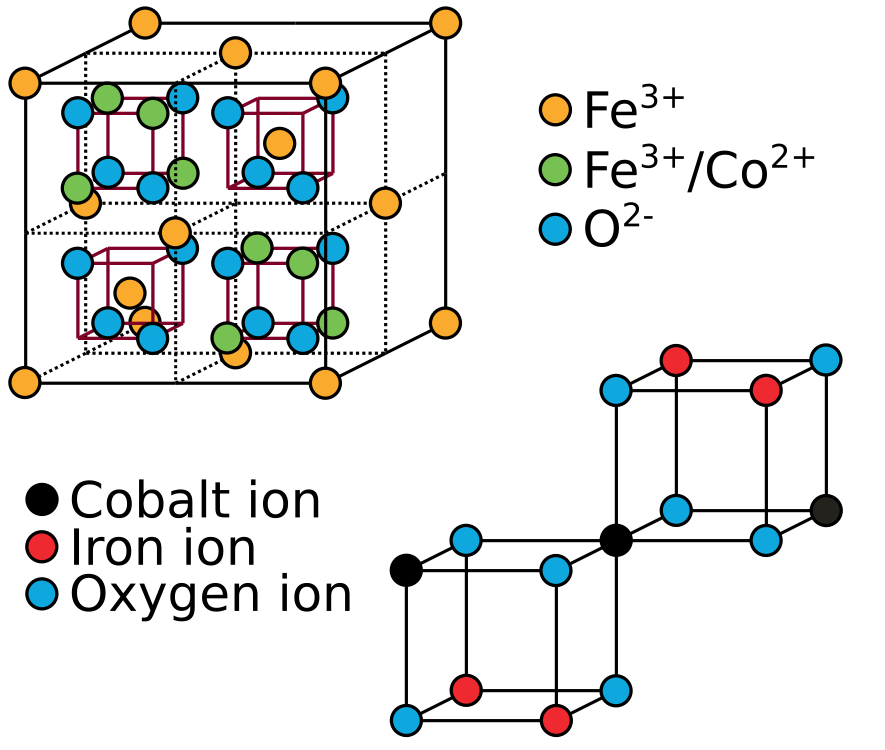
\includegraphics{ferrite_cobaltFerriteStructure}
    \caption{\label{fig:theoreticalBackground:ferrites:cofe2o4Structure}Unit cell of the spinell structure \ch{AB2O4} (upper image) \cite{Sickafus_1999_Struc} and focus on a neighborhood of a cobalt ion (lower image) \cite{Tachiki_1960_Origi}. The bordeaux small cubes in the unit cell repeat in the back and are not shown for clarity.}
  \end{figure}

  \ch{CoFe2O4} ideally crystallizes in the inverse spinell structure, which has the space group Fd-3m (No. 227).
  Here, the oxygen atoms form a close cubic packing with eight tetrahedral and four octahedral interstices per formula unit \cite{Sickafus_1999_Struc}.
  In the normal spinell structure \ch{AB2O4} the \ch{A} cation occupy 1/8 of the tetrahedral ($T_d$) and the \ch{B} cations 1/2 of the octahedral ($O_h$) interstices.
  The unit cell is shown in \reffig{fig:theoreticalBackground:ferrites:cofe2o4Structure} (upper image), which contains eight formula units and has a lattice parameter for cobalt ferrite in the order of $a \eq 8.38 \unit{\angstrom}$ \cite{Goldman_1999_Cryst}.
  In the inverse spinell case, the \ch{A} atoms are found in one half of the $O_h$ sites, while the \ch{B} atoms occupy both the $T_d$ and the other half of the $O_h$ sites.
  Therefore, the inverse spinell is commonly noted as \ch{B[AB]O4}, where the square brackets denote those atoms that occupy the octahedral positions.

  In the case of cobalt ferrite, it was shown that the magnetic moment and high anisotropy constant can be explained broadly by considering only the Hamiltonian of a cobalt ion and its crystal field \cite{Slonczewski_1958_Origi, Tachiki_1960_Origi}.
  From this theory, it is shown that the deduced magnitude and temperature dependence of the cubic anisotropy constant $K_1$ reproduces the experimental result obtained from torque measurements on bulk crystals \cite{Shenker_1957_Magne}
  \begin{align}
    K_1 \eq 1.96 \cdot 10^6 \exp(-1.90 \cdot 10^{-5} T^2) \unit{\frac{J}{m^3}},
  \end{align}
  and the magnetic moment per cobalt ion in cobalt ferrite is derived to be approximately $\mu_\textsf{Co} \eq 3.5 \mu_B$, where experimental values range is cited to be from $3.3 \mu_B - 3.9 \mu_B$ \cite{Tachiki_1960_Origi}.
  With the lattice parameter this magnetic moment corresponds to a saturation magnetization of
  \begin{align}
    M_s \eq 8\mu_\textsf{Co}/a^3 \eq 450 \unit{kAm^{-1}}.
  \end{align}

  Interactions between cobalt and iron ... superexchange ... double-exchange mechanism

  Detailed studies of the iron atom occupation via M\"ossbauer spectroscopy in a magnetic field show that in actual bulk cobalt ferrite crystals, the structure is more of a mixed inverse spinell structure, where the iron occupation is not 1:1 in $T_d$ and $O_h$ positions, but depending on the sample preparation, more iron atoms can shift to the octahedral positions and thus cobalt atoms also occupy the tetrahedral interstices \cite{Sawatzky_1968_Catio, Sawatzky_1969_Mossb}.
  In the case of nanoparticular cobalt ferrite, the relative content of cobalt and iron in the spinell structure, as well as the relative occupation of the sites varies broadly depending on the preparation process and the particle size \cite{Muscas_2015_Evolu, Repko_2015_Oleate, Peddis_2008_Spinc} and has to be studied on a case to case basis.









\end{document}